
%(BEGIN_QUESTION)
% Copyright 2011, Tony R. Kuphaldt, released under the Creative Commons Attribution License (v 1.0)
% This means you may do almost anything with this work of mine, so long as you give me proper credit

Examine the loop diagram for a laboratory gasoline flow control system:

$$\includegraphics[width=15.5cm]{i03422x01.eps}$$

This system used to work just fine, but now it has a problem: the controller registers zero flow.  Your first diagnostic step is to check to see if there actually is gasoline flow through the flowmeter and valve by looking at the rotameter.  You see that the rotameter shows no flow as well.

Identify two possible faults in this system that could account for the controller's condition and the rotameter's indication:

\begin{itemize}
\item{} Possible fault:
\vskip 10pt
\item{} Possible fault:
\end{itemize}

\underbar{file i03422}
%(END_QUESTION)





%(BEGIN_ANSWER)

5 points for each correct answer:

\vskip 10pt

(Any faults that account for the lack of flow while still enabling the flow transmitter and rotameter to agree with each other).

%(END_ANSWER)





%(BEGIN_NOTES)

{\bf This question is intended for exams only and not worksheets!}.

%(END_NOTES)


